
\chapter{Gestione Memoria Principale}
Abbiamo già visto nei capitoli precedenti l'importanza della memoria principale nella gestione dei processi. Il sistema operativo ha il compito di gestirla in modo efficiente così da permettere l'esecuzione dei programmi.

\section{Introduzione}
Alla compilazione di un programma il compilatore genera un modulo oggetto dove tutti gli indirizzi sono in \textbf{riferimento} a quello dell'inizio del modulo. Questo significa che c'è libertà di inserire il processo in qualsiasi punto della memoria e ci sono quindi decisioni che il sistema operativo è responsabile di prendere.

\spacer
Per mantenere la sicurezza dei dati è importante che ogni processo possa accedere solamente ai dati ad esso assegnati, per questo motivo assegniamo ad ogni processo due indirizzi logici, uno base ed uno limite. Ora il processo può accedere solo agli indirizzi tali che $base \le indirizzo \le base+limite$.

\begin{figure}[H]
    \centering
    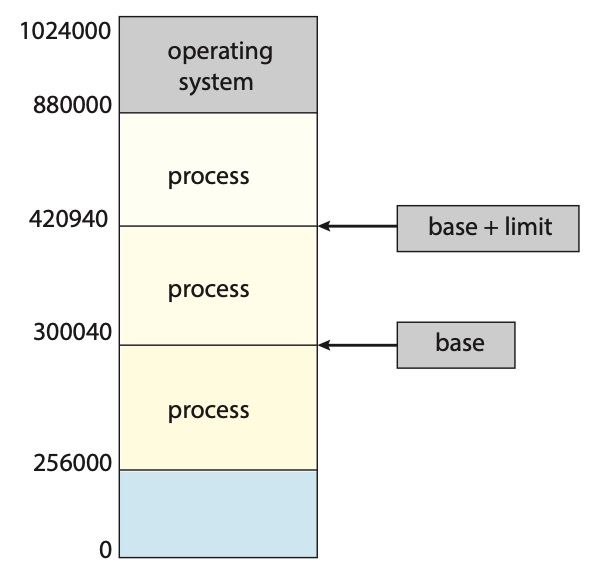
\includegraphics[width=0.3\linewidth]{assets/base-limit-memory.jpg}
\end{figure}

Nei sistemi moderni il processo può essere rilocato nella memoria a \textit{runtime}, questo grazie all'utilizzo della memoria virtuale. Questo ci permette di tradurre gli indirizzi fisici della memoria in indirizzi virtuali, non è quindi necessario allocare ad un programma un segmento contiguo di memoria, ma è possibile rendere contigui segmenti fisicamente lontani in memoria.

Questa traduzione avviene a livello hardware da parte della memory mapping and managment unit (MMU).

\begin{figure}[H]
    \centering
    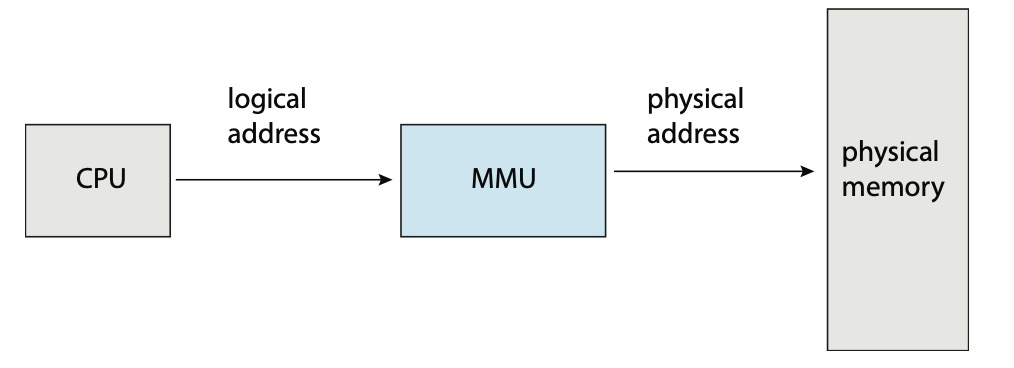
\includegraphics[width=0.45\linewidth]{assets/MMU.jpg}
\end{figure}

\subsubsection*{File di Paging}
Una funzionalità introdotta da Windows XP, che estende la memoria RAM del sistema con un file presente in memoria secondaria, delle stesse dimensioni.

\subsection{Frammentazione}
L'allocazione e la rimozione della memoria comporta la frammentazione della memoria.
\begin{sitemize}
    \item La \textbf{frammentazione interna}, quando la memoria allocata ad ogni programma è leggermente maggiore di quella richiesta.
    \item La \textbf{frammentazione esterna}, quando lo spazio per un nuovo processo è disponibile, ma non è contiguo, in questo caso può essere necessario rilocare dei processi per compattare lo spazio libero.
\end{sitemize}

\section{Paginazione}
La paginazione risolve il problema posto dalla frammentazione esterna consentendo la non contiguità degli indirizzi fisici, mantenendo invece la contiguità negli indirizzi logici.

\subsection{Implementazione}
Si divide la memoria fisica in blocchi di dimensione fissa, detti frame o pagine fisiche. Allo stesso modo si divide anche la memoria logica in blocchi della stessa dimensione.

La \textbf{tabella delle pagine}, tiene traccia delle relazioni tra memoria fisica e logica e tiene traccia delle pagine libere.

\spacer
Gli indirizzo logici generati dalla CPU vengono suddivisi in:
\begin{sitemize}
    \item \textbf{Numero di pagina:} indice che verrà usato nella tabella delle pagine.
    \item \textbf{Offset nella pagina:} definisce l'offset a partire dall'inizio della pagina
\end{sitemize}

\begin{figure}[H]
    \centering
    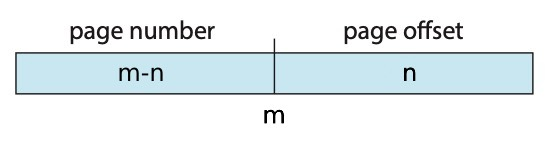
\includegraphics[width=0.35\linewidth]{assets/page-number-offset.jpg}
\end{figure}

Se lo spazio logico ha dimensione $2^m$ allora si hanno $2^{m-n}$ pagine di dimensione $2^n$. La scelta di m ed n detta anche la dimensione della tabella delle pagine.

\begin{figure}[H]
    \centering
    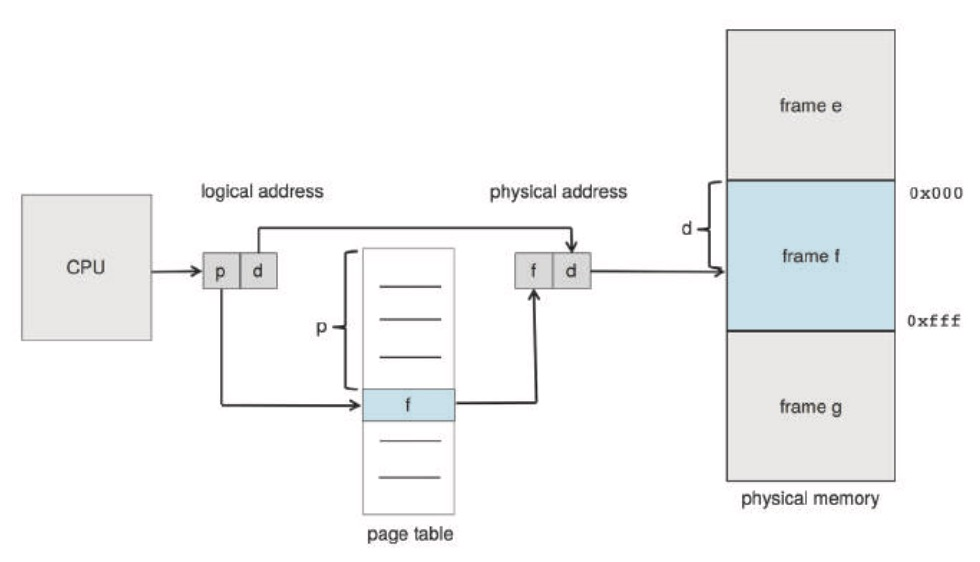
\includegraphics[width=0.48\linewidth]{assets/paginazione.jpg}
\end{figure}

\subsubsection*{Frammentazione}
Si ottiene della frammentazione interna quando un processo non occupa completamente un frame, ad esempio un processo di 72766 byte occupa 36 pagine da 2048 byte, ma l'ultima pagina viene riempita circa a metà.

\subsubsection*{Dimensioni dei frame}
Un'importante considerazione che deve essere fatta nell'architettura dell'elaboratore è la dimensione delle pagine.

Pagine più piccole permettono una minore frammentazione in quanto si possono meglio adattare alle dimensioni del programma, esse migliorano inoltre il principio di località.

Al contrario pagine più grandi riducono le dimensioni della page table e riducono il numero di page fault incontrati.

La soluzione adottata da molti sistemi operativi è quella di costruire pagine di diverse dimensioni così da potersi adattare ad ogni processo.

\subsubsection*{Pagine Bloccate}
In alcuni casi occorre mantenere delle pagine perennemente in memoria, come nel caso di operazioni di I/O tramite DMA, per questo motivo è possibile segnalare al pager delle pagine bloccate (\textit{pinned}) che non possono essere selezionate come vittime dall'algoritmo di sostituzione.

\subsection{Supporto Hardware}
Si utilizza una tabella delle pagine per ogni processo, essa risiede nella memoria principale e il processo ha un puntatore ad essa (PTBR) ed alla sua lunghezza (PTLR).

\spacer
Uno degli svantaggi di inserire la tabella delle pagine nella memoria principale è l'\textbf{aumento del tempo di accesso dati}, infatti per ogni richiesta devono essere fatte due richieste alla memoria, una alla tabella ad una all'indirizzo fisico.

\spacer
Una soluzione è il \textit{translation look-aside buffer (TLB)} che permette la ricerca in parallelo su una piccola tabella (64-1024 elementi). Essa può essere utilizzata come cache per la tabella delle pagine.

La TLB è più efficiente e sicura quando non viene condivisa tra più processi, ad ogni \textit{context switch} andrebbe fatto un \textit{flush} della memoria.
È possibile aggiungere un valore \textit{Address Space IDentifier (ASID)} che identifica il processo a cui appartiene l'associazione, questo permette di mantenere la TLB di un processo anche in un context switch.

\begin{figure}[H]
    \centering
    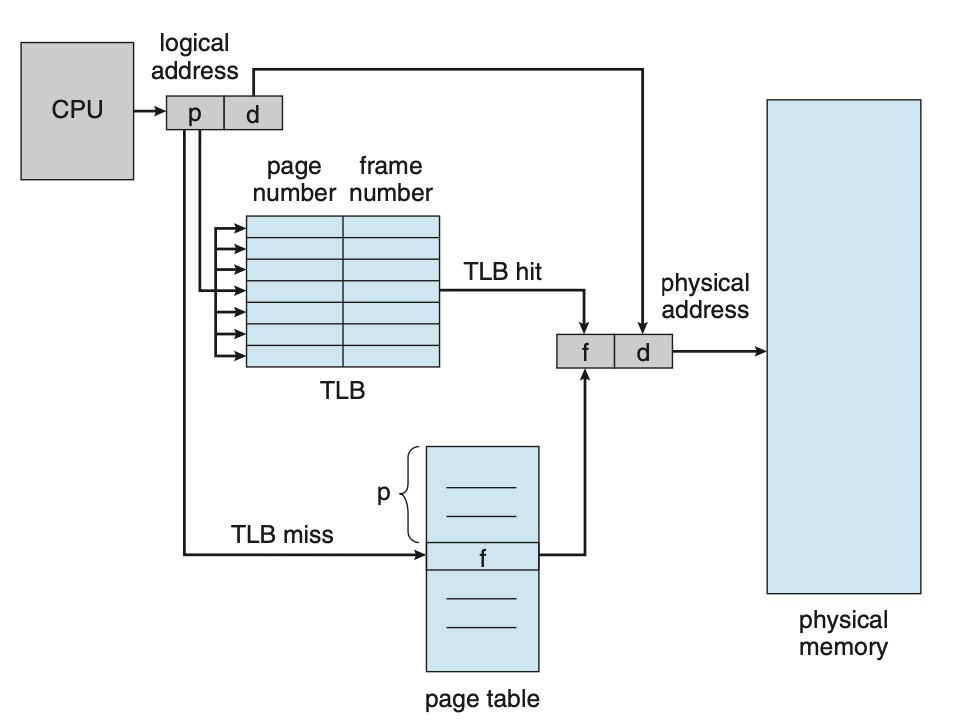
\includegraphics[width=0.5\linewidth]{assets/paginazione-tlb.jpg}
\end{figure}

\subsubsection{Page Fault}
Se un processo fa riferimento ad una pagina che al momento non è in memoria principale viene generato un \textbf{interrupt} di tipo page fault.

Il processo viene quindi sospeso finché il sistema operativo non carica la pagina mancante in memoria principale. Se la memoria è piena è necessario utilizzare un algoritmo di camnio pagina per scegliere quale pagina rimuovere.

\subsubsection{Protezione della Memoria}
Viene implementata grazie ad uno o più \textbf{bit di protezione} che determinano se una è possibile accedere una determinata pagina in lettura oppure lettura/scrittura.

\spacer
Inoltre viene aggiunto un \textbf{bit di validità}, esso permette di individuare le pagine che non appartengono agli indirizzi \textit{logici} del processo, questo viene poi segnalato all'utente tramite un'interrupt.

\subsection{Dimensioni della Tabella}
La tabella delle pagine può arrivare facilmente a dimensioni importanti, soprattutto quando se ne crea una per ogni processo, una rappresentazione naturale, ma inefficiente.

\subsubsection*{Tabella delle Pagine Invertita}
Una soluzione è costruire una tabella delle pagine invertita, la quale ha un elemento per ogni frame fisico e salva il frame logico e un identificatore del processo.


Questo riduce lo spazio totale usato dalle tabelle delle pagine ma incrementa il tempo di ricerca nella tabella.
Inoltre rende difficile la condivisione delle pagine fisiche tra processi.

\begin{figure}[H]
    \centering
    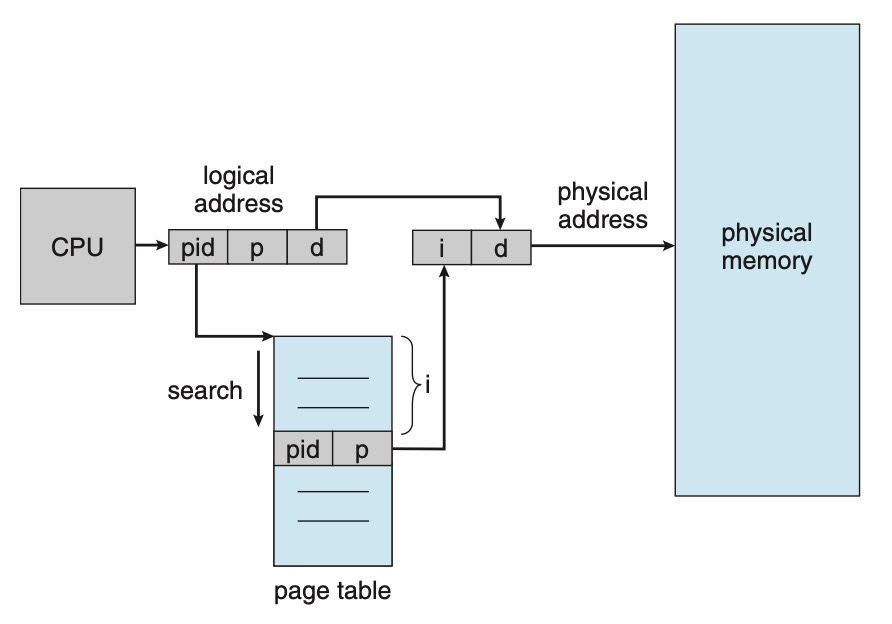
\includegraphics[width=0.45\linewidth]{assets/tabella-pagine-invertita.jpg}
\end{figure}

\subsubsection*{Paginazione Gerarchica}
L'idea con questa soluzione è quello di dividere lo spazio degli indirizzi logici in più tabelle delle pagine. Il caso più semplice è quello ottenuto utilizzando una paginazione a due livelli.

\begin{figure}[H]
    \centering
    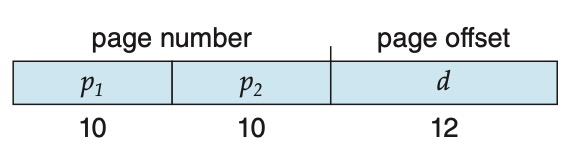
\includegraphics[width=0.35\linewidth]{assets/paginazione-doppia.jpg}
\end{figure}

$p_1$ viene utilizzato per indicizzare la tabella delle tabelle, mentre $p_2$ per indicizzare la tabella delle pagine.

\begin{figure}[H]
    \centering
    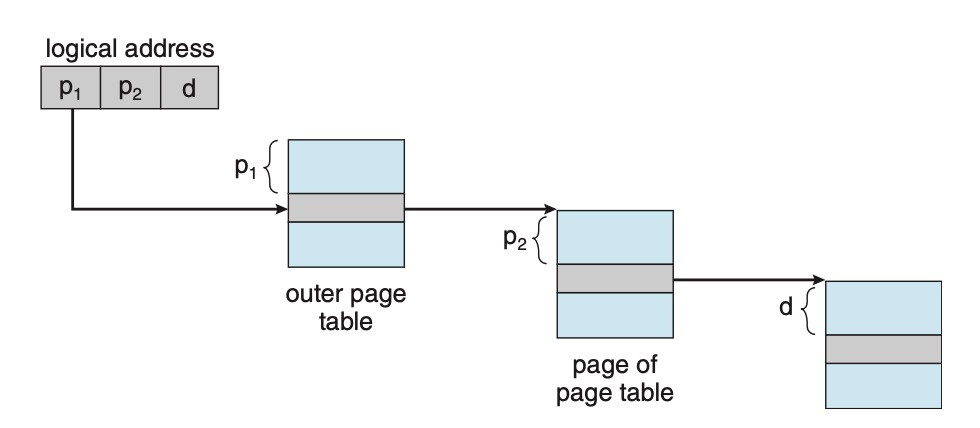
\includegraphics[width=0.5\linewidth]{assets/paginazione-gerarchica.jpg}
\end{figure}

Per le architetture a 64 bit questo tipo di paginazione necessita di troppi livelli di paginazione, è quindi da considerarsi inadeguata.

\subsubsection*{Tabella delle Pagine Hash}
Comunemente utilizzato per architetture a 64 bit.

L'elemento che viene inserito nella funzione di hash è il numero della pagina virtuale. Gli elementi della tabella sono liste concatenate, questo per gestire le eventuali collisioni dovute alla funzione di hash.

\spacer

In particolare ciascun elemento della tabella è composto da:
\begin{sitemize}
    \item Numero della pagina virtuale
    \item Numero della pagina fisica
    \item Puntatore al frame successivo
\end{sitemize}

\begin{figure}[H]
    \centering
    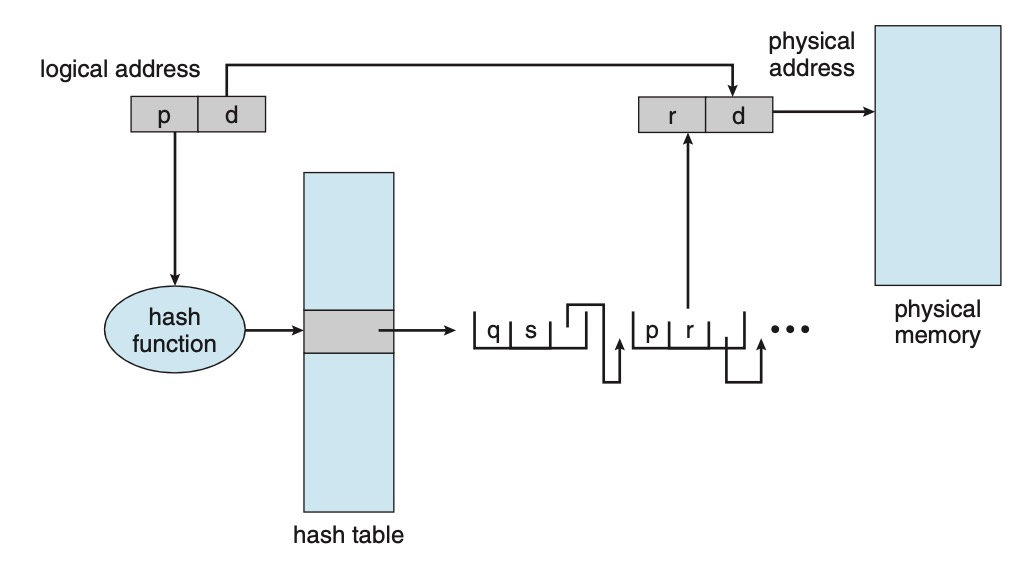
\includegraphics[width=0.5\linewidth]{assets/hashed-page-table.jpg}
\end{figure}

\begin{note}
    Per gli spazi a 64 bit si utilizza una tabella delle pagine a gruppi, ovvero una tabella hash dove ogni elemento contiene riferimenti alle pagine fisiche corrispondenti ad un gruppo di pagine virtuali contigue.
\end{note}

\subsubsection*{Segmentazione}
Gestisce la memoria in segmenti di dimensione variabile, questo è più vicino a come l'utente immagina l'organizzazione della memoria. Ogni segmento è un'unità logica:
\begin{sitemize}
    \item Procedure e funzioni
    \item Variabili
    \item Oggetti
\end{sitemize}

Si ha quindi una \textbf{tabella dei segmenti} per ogni processo che mappa gli indirizzi logici in coppie base, limite.

\begin{figure}[H]
    \centering
    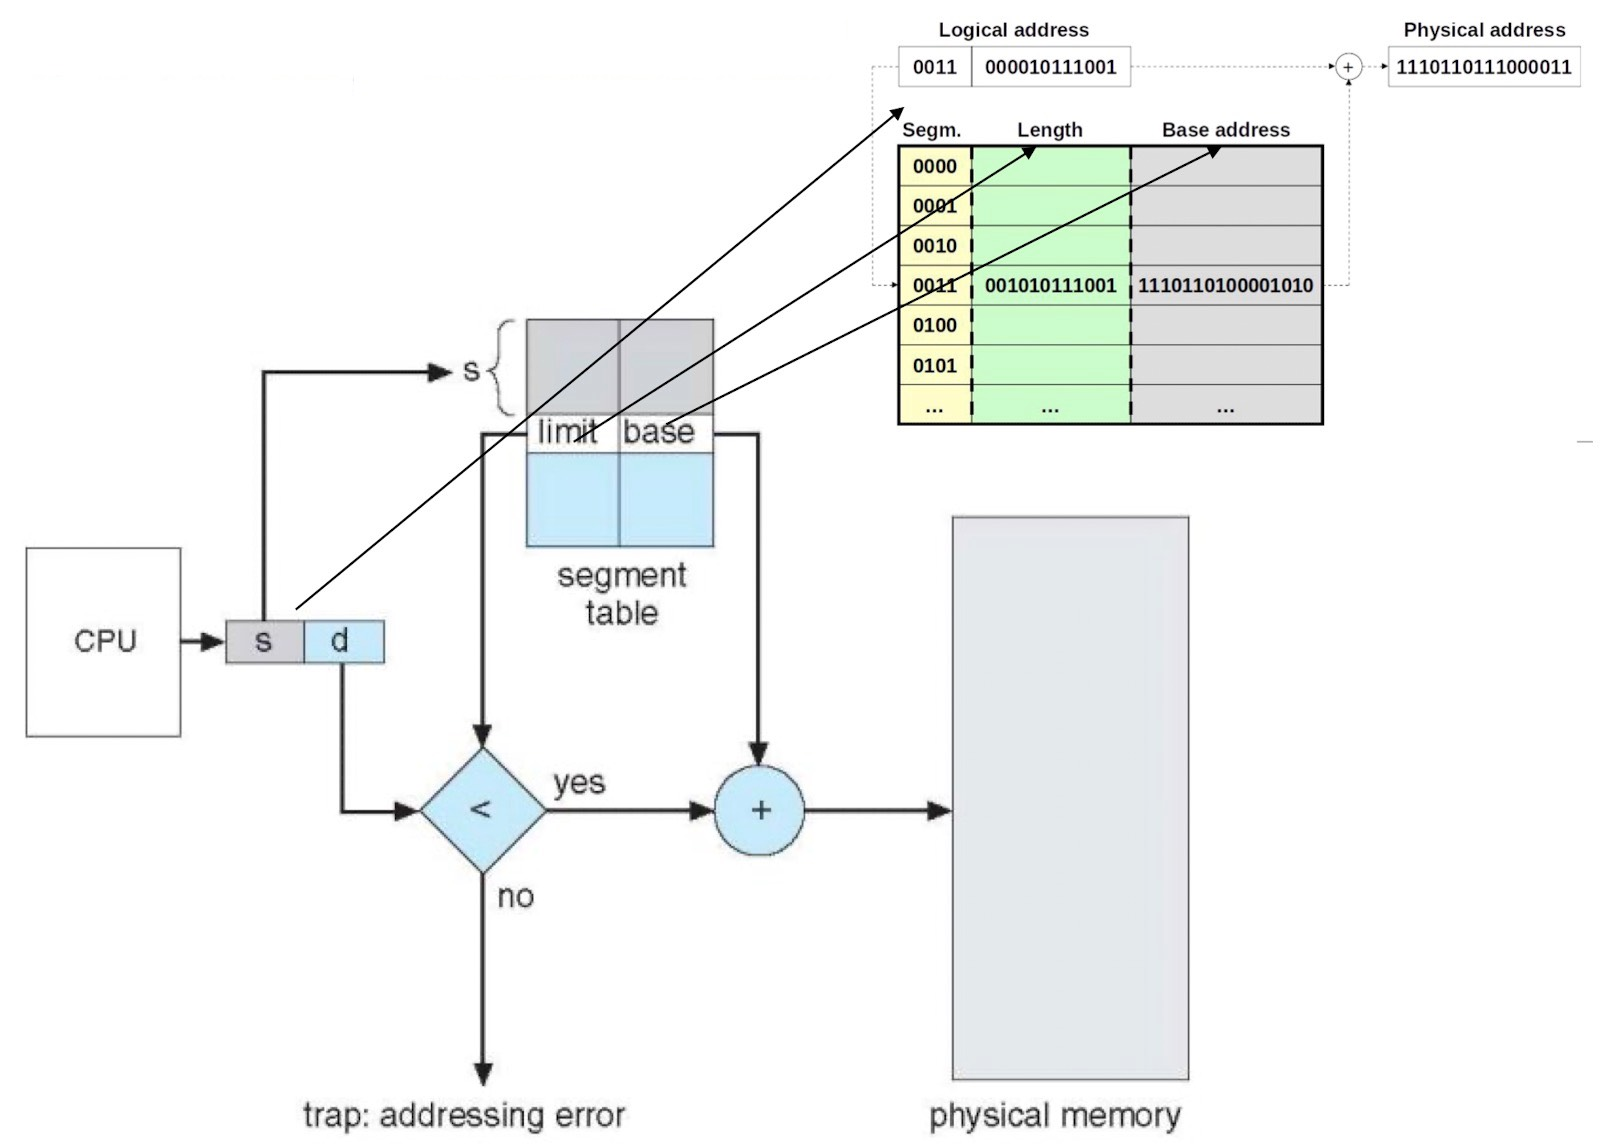
\includegraphics[width=0.48\linewidth]{assets/segmentazione.jpg}
\end{figure}

Due registri sono di particolare importanza in questo caso: STRB (\textit{Segment Table Base Register}) e STLR (\textit{Segment Table Length Register}).

\subsection{Implementazioni}
\subsubsection{Intel 32}
Il pentium supporta sia la segmentazione pura che la segmentazione mista a paginazione.

\begin{figure}[H]
    \centering
    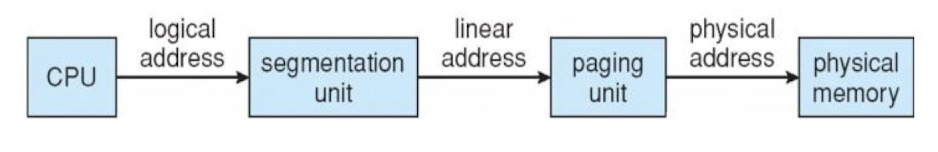
\includegraphics[width=0.5\linewidth]{assets/architettura-memoria-pentium.jpg}
\end{figure}

I segmenti possono essere di dimensione variabile, fino a 64 Kbyte, e possono essere al massimo $16 K$ per processo, di questi al massimo $8 K$ possono essere privati (Informazioni nella \textit{Local Descriptor Table, LDT}) e altri $8 K$ condivisi (Informazioni nella \textit{Global Descriptor Table, GDT}).

Il selettore è di 16 bit, dove 13 bit rappresentano l'indice del segmento ($2^{13} = 8192$), 1 bit per indicare LDT o GDT e 2 bit di protezione.
Altri 16 bit sono di offset.

\begin{figure}[H]
    \centering
    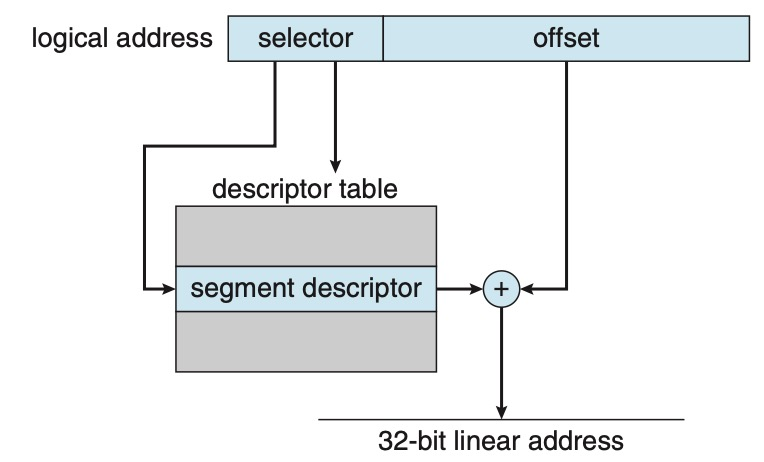
\includegraphics[width=0.5\linewidth]{assets/pentium-segmentation.jpg}
\end{figure}

Nella tabella vengono salvate anche altre informazioni, come un bit per indicare se il segmento è in memoria principale e uno per indicare se è stato modificato.

L'indirizzo ottenuto dalla segmentazione può essere paginato. Le pagine per il pentium possono essere di 4MB (1 livello) o 4KB (2 livelli) e viene usata una paginazione a due livelli.

\begin{figure}[H]
    \centering
    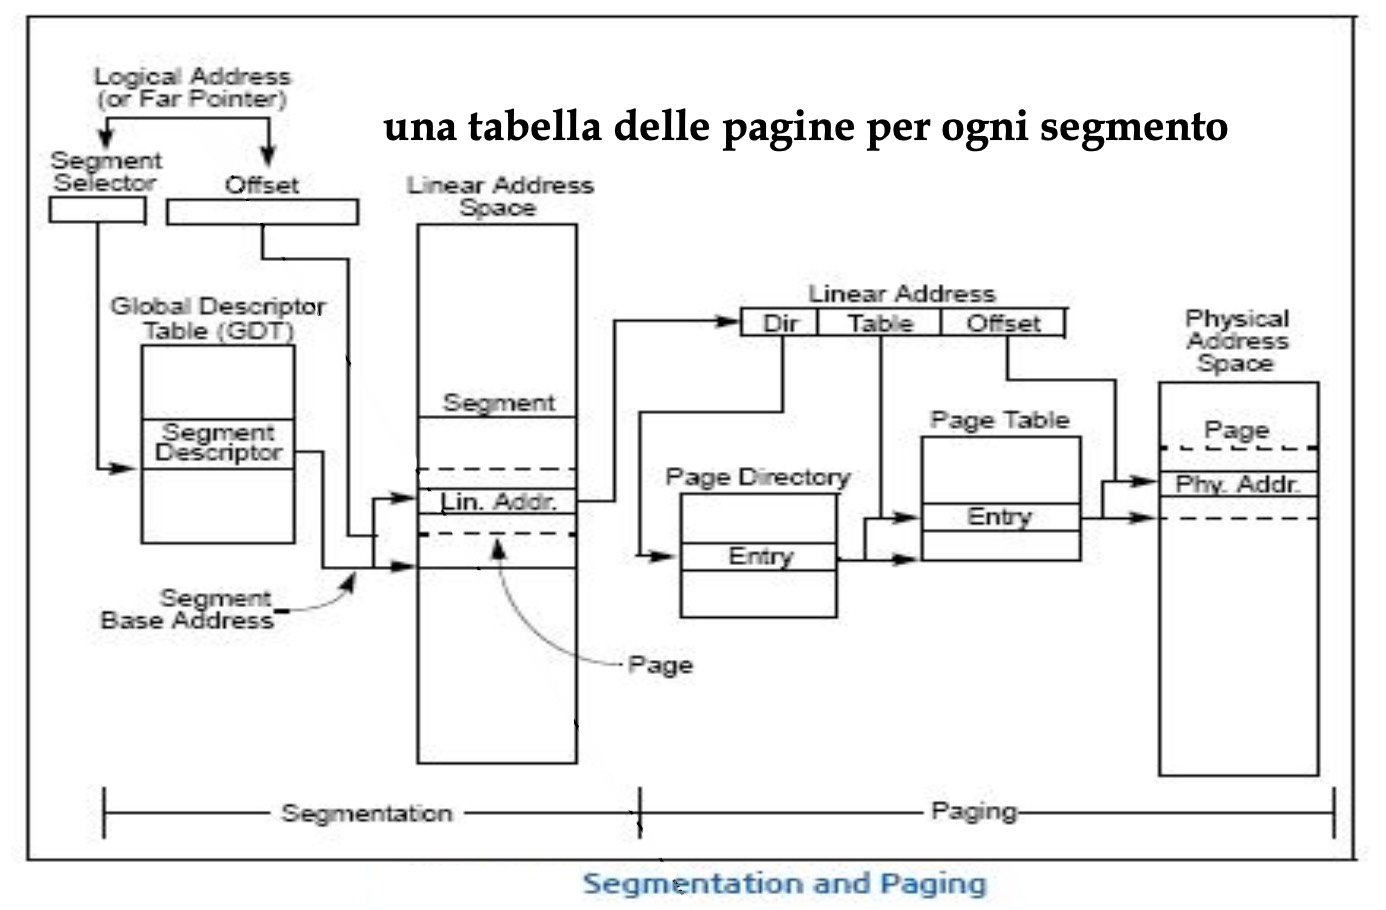
\includegraphics[width=0.5\linewidth]{assets/intel32-3.jpg}
\end{figure}

La dimensione della descriptor table viene aumentata nel tempo, prima a 24 e poi a 32 bit

\subsubsection{PAE}
Anche detto \textbf{Page Address Extension}, permette di raggiungere i 64 Gbyte di memoria.

Le principali modifiche all'architettura sono due: Viene inserito un ulteriore livello di paginazione, una page directory pointer table di 4 elementi e gli elementi della descriptor table arrivano a 64 bit, di cui solo 36 vengono utilizzati, arrivando così ad indicizzare 64 Gbyte di memoria.

\spacer
Le singole applicazioni possono, in generale, accedere solamente a 4GB di memoria, ma esse possono essere inserite in 64 Gbyte di memoria.

Inoltre è possibile per le applicazioni utilizzare delle system call per spostare il proprio spazio di indicizzazione, permettendo così di accedere ad una maggiore quantità di memoria RAM.

\begin{figure}[H]
    \centering
    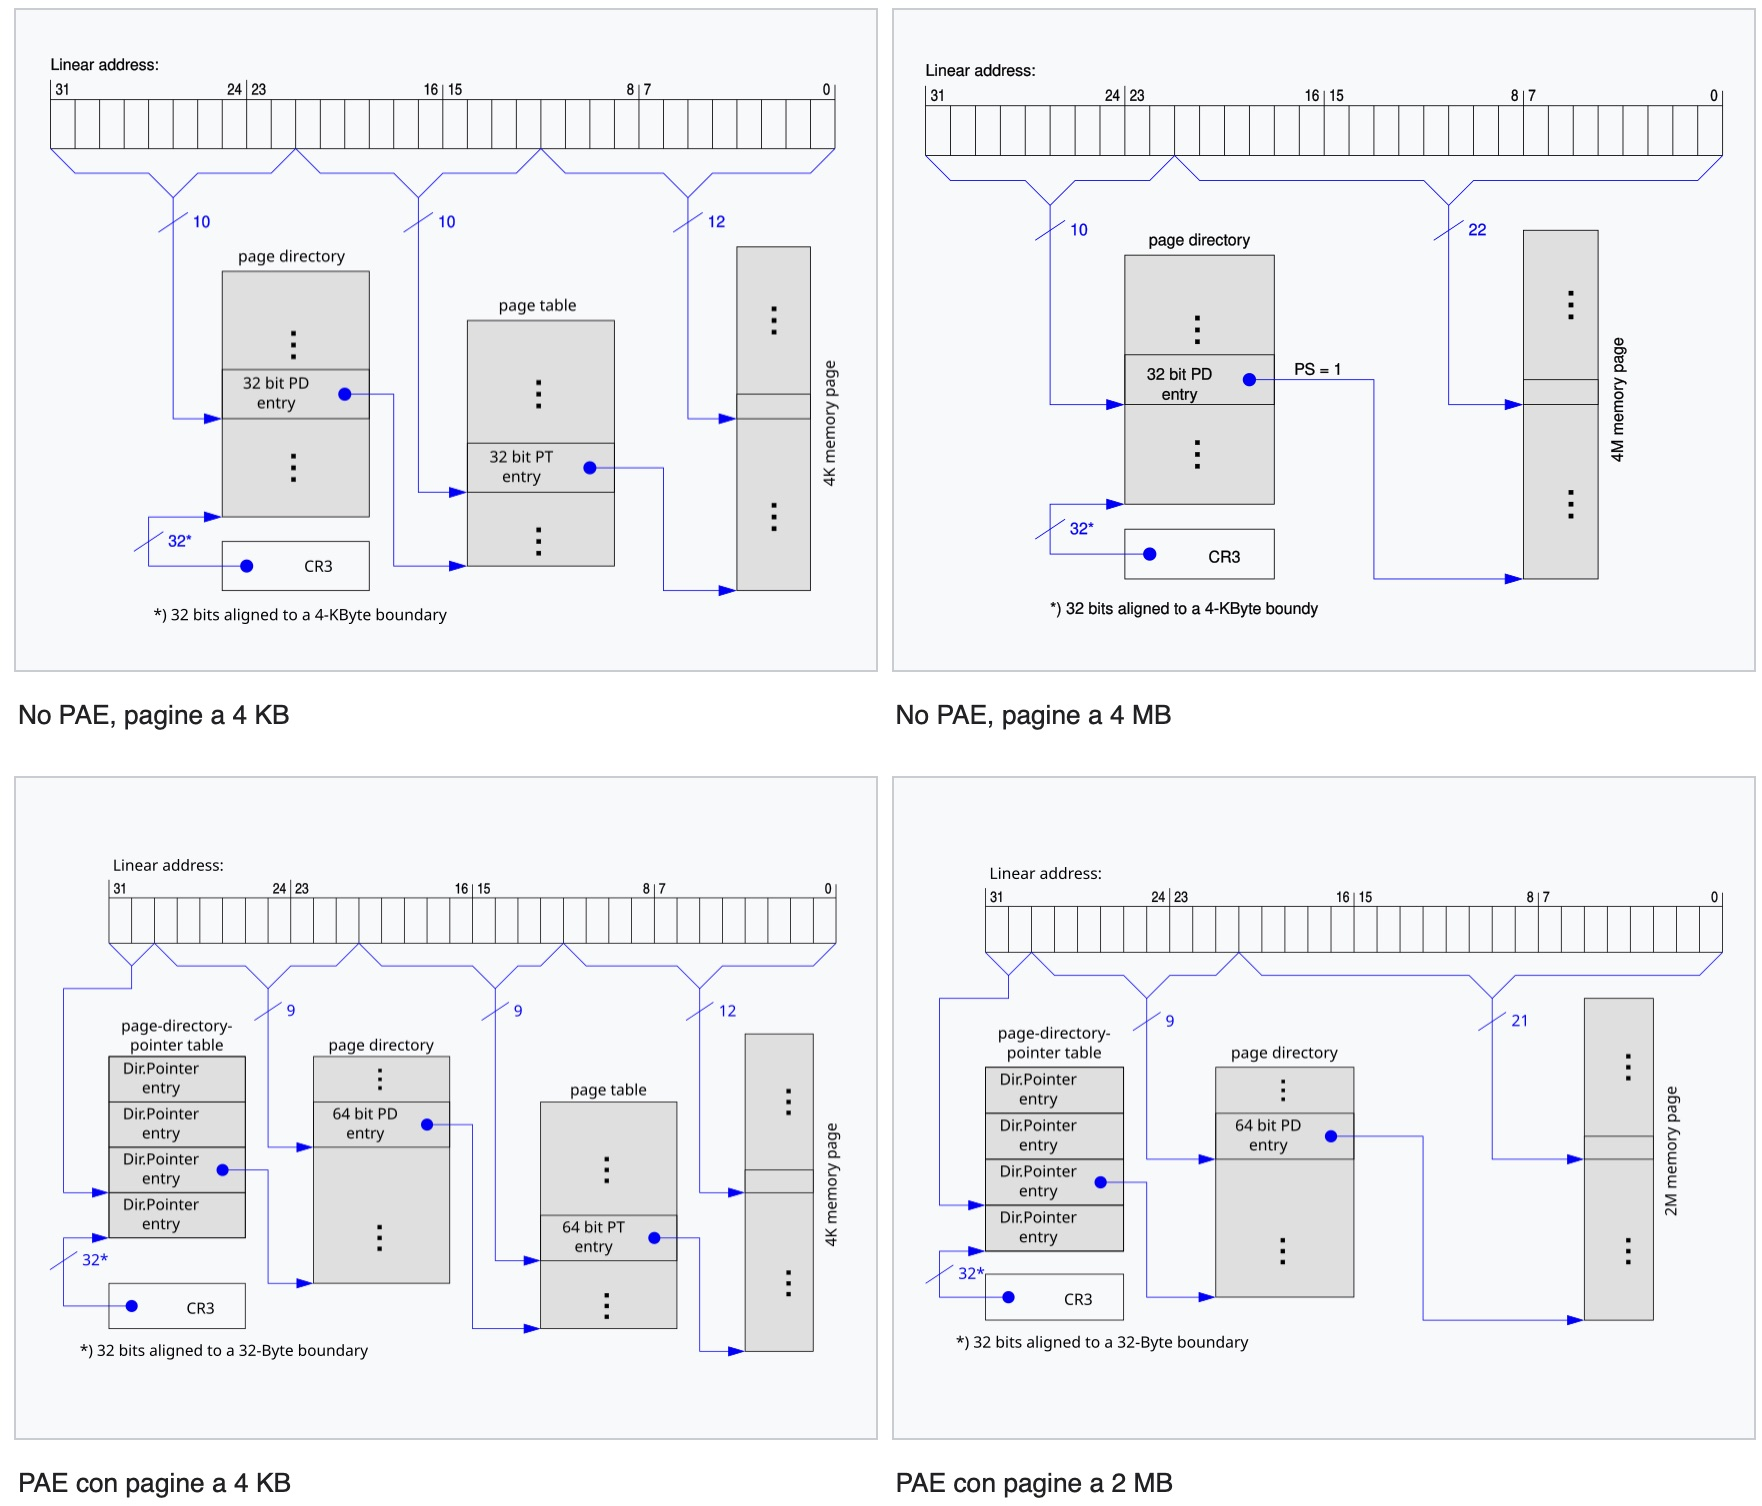
\includegraphics[width=0.75\linewidth]{assets/pae.jpeg}
\end{figure}

\subsubsection{Intel x86-64}
Nei sistemi a 64 bit in realtà non se ne usano così tanti ($2^{64} = 17,179,869,184$ GB), gli indici sono tutti a 48 bit, lasciando inutilizzati i primi 16 bit.

L'architettura supporta pagine da 4KB, 2MB, 1GB.

\begin{figure}[H]
    \centering
    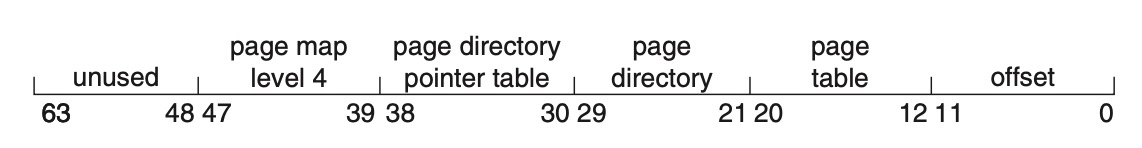
\includegraphics[width=0.6\linewidth]{assets/x64-address.jpg}
\end{figure}

È possibile utilizzare la PAE anche qui con l'obiettivo di portare gli indirizzi fisici da 48 a 52 bit.

\subsubsection{ARMv8}
Anche i processori ARM lavorano su 64 bit ed anche loro utilizzano fino a 4 livelli di paging ottenendo così pagine da 4KB, 2MB, 1GB.

\begin{figure}[H]
    \centering
    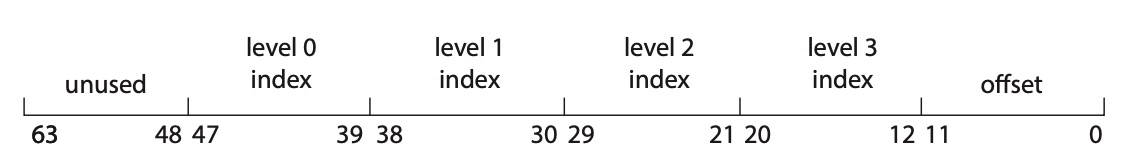
\includegraphics[width=0.6\linewidth]{assets/arm-address.jpg}
\end{figure}

\section{Memoria Virtuale}
Abbiamo visto come la paginazione può permettere di condividere la memoria tra più processi, tuttavia è raro che un intero processo venga inserito nella memoria principale prima che venga eseguito.

Questo perché non tutte le sezioni del programma vengono eseguite allo stesso tempo, è quindi conveniente caricarle in modo dinamico.

\spacer
In questo modo le dimensioni totali del programma non sono più limitate dalle dimensioni della memoria fisica e viene lasciato più spazio nella memoria per la multiprogrammazione.

Inoltre l'utilizzo della memoria virtuale rende più semplice la condivisione di librerie o dati.

\subsection{Spazio degli Indirizzi Virtuali}
La memoria virtuale separa la memoria logica utilizzata dagli sviluppatori da quella fisica, rendendo così più semplice il lavoro del programmatore che non deve gestire manualmente le limitazioni fisiche della memoria principale.

\spacer

Nello spazio degli indirizzi virtuali i programmi sono allocati in modo contiguo, a partire da un certo indirizzo iniziale $0$ fino a quello finale $Max$.

Nella memoria fisica invece il programma può essere allocato in pagine sparse. La MMU si occupa della conversione degli indirizzi logici in fisici.

\spacer
Condividere librerie è ora estremamente semplice, basterà mappare le pagine logiche agli stessi frame fisici.

In questo modo entrambi i processi vedono gli indirizzi della libreria comune come propri, ma in realtà i dati non vengono duplicati.

\section{Pager}
Un vantaggio della memoria virtuale è quello di poter caricare in modo dinamico i frame fisici dalla memoria secondaria. Il modulo del sistema operativo che si occupa della paginazione su richiesta è il \textit{pager}.

\spacer
Il termine \textit{swapping} indica l'atto di inserire o rimuovere delle pagine dalla memoria.
Quando una pagina viene rimossa dalla memoria essa viene riportata in un dispositivo di memroia secondaria, all'interno di un file (Windows) o una partizione (linux)

\spacer
Spesso si utilizza uno swapper pigro, che carica le pagine in RAM solo quando esse vengono richieste.

\begin{note}
    Inoltre spesso si utilizza una partizione di swap sulla memoria secondaria per ampliare ulteriormente le dimensioni della memoria principale, essa permette di ottenere delle prestazioni migliori in quanto non incorre nella frammentazione dei dischi.
\end{note}

Per sapere quali pagine si trovano già in memoria e quali invece devono essere caricate il pager utilizza una tabella delle pagine, essa associa la memoria logica a quella fisica. Inoltre comprende un bit di validità che specifica se il frame si trova in memoria o meno.

\begin{figure}[H]
    \centering
    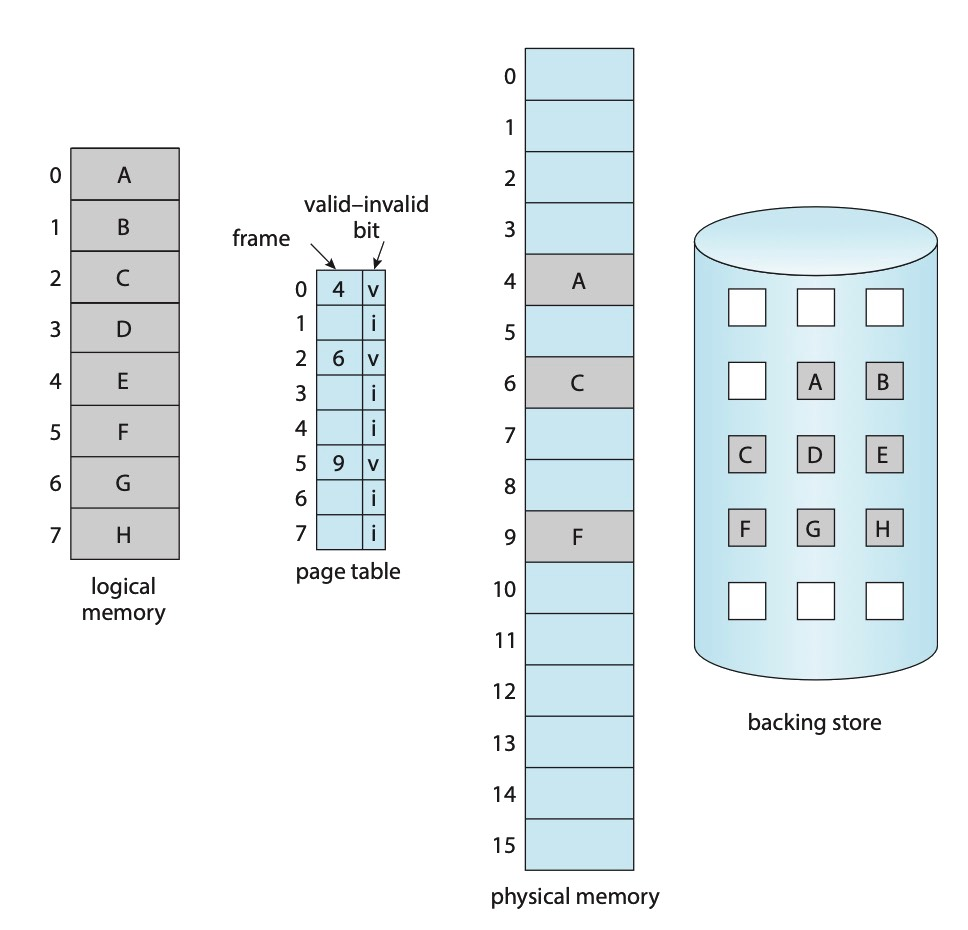
\includegraphics[width=0.45\linewidth]{assets/tabella-pagine.jpg}
\end{figure}

\subsection{Page Fault}

Quando il programma richiede un indirizzo appartenente ad una pagina non caricata in memoria causa una trap al sistema operativo, una \textit{page fault}.

A questo punto il sistema operativo consulta una sua tabella delle pagine e invia al programma un abort se l'indirizzo non è valido.

Se viene trovata la pagina nella memoria secondaria allora essa viene caricata nella RAM e l'esecuzione del programma può riprendere.

\begin{figure}[H]
    \centering
    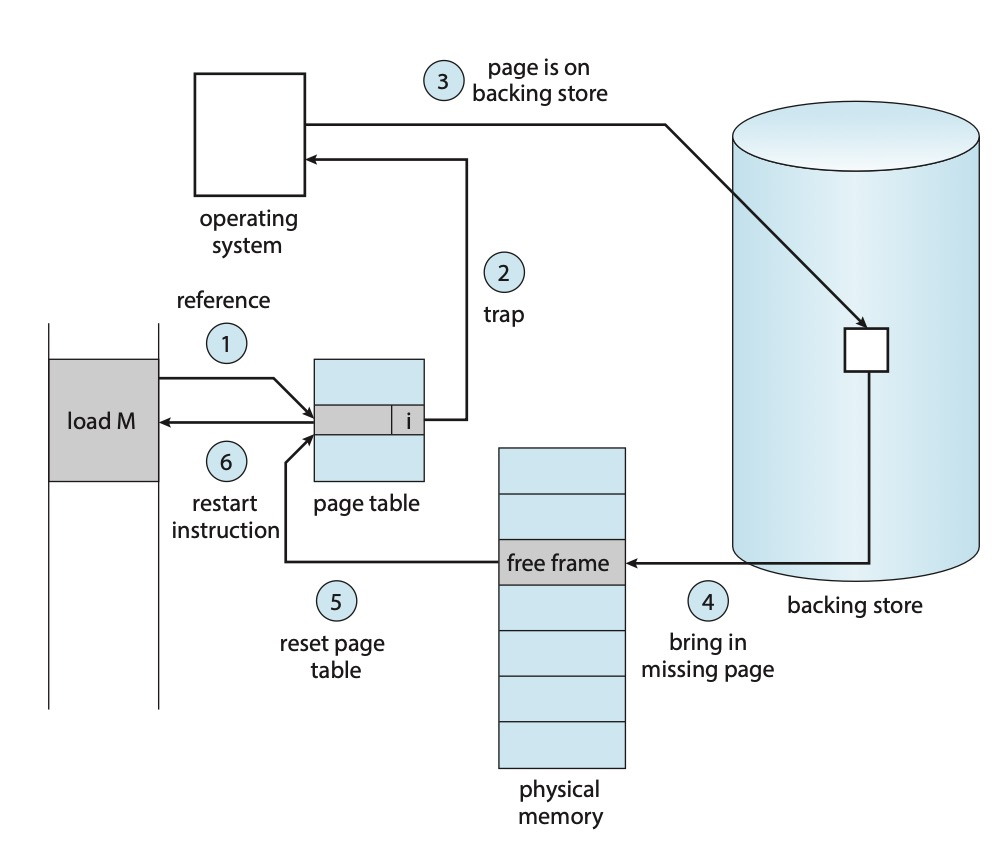
\includegraphics[width=0.5\linewidth]{assets/gestione-page-fault.jpg}
\end{figure}

Se non sono disponibili dei frame liberi nella memoria principale sarà necessario rimuovere prima una pagina secondo un algoritmo di selezione.
Si ricerca un algoritmo che riduca al minimo il numero di page fault in quanto esse sono un fattore importante sulle prestazioni del sistema.

\spacer
Viene impiegato un bit di modifica, o \textit{dirty bit}, per ridurre l'overhead dei trasferimenti di pagine. Solo le pagine modificate vengono riscritte al disco, le altre possono essere semplicemente sovrascritte.

\subsubsection{Prestazioni}
Il tempo effettivo di accesso alla memoria (EAT) si può calcolare nel seguente modo:
$$EAT = (1 - p)\cdot \text{accesso alla memoria} + p \cdot \text{overhead page fault}$$

Dove p è la probabilità di ottenere un page fault.

\spacer
Assumendo dei valori realistici, il tempo di acccesso alla memoria è di circa 200ns, mentre l'overhead per un page fault 8ms.

Sotto queste ipotesi se si ha un page fault ogni 1000 accessi l'accesso alla memoria viene mediamente rallentato di un fattore di 40.

Per ottenere un fattore di rallentamento accettabile (<0.1) è necessario arrivare ad un page fault ogni 400,000 richieste.

\subsection{Prepaging}
Per ridurre il gran numero di page fault che avvengono all'avvio del processo si può utilizzare il prepaging, ovvero si possono copiare un certo numero di pagine in memoria prima dell'esecuzione del programma.

\spacer
Ad esempio, se un programma è stato sospeso per una richiesta I/O, quando esso riprende l'esecuzione è possibile riportare in memoria il suo ultimo working set.

\spacer
È importante bilanciare le prestazioni di questa operazione ed assicurarsi che il vantaggio in riduzione di page fault sia superiore al costo di prepaging.

\subsection{Algoritmi di Paging}
Il paging richiede diversi algoritmi per un funzionamento corretto, in particolare sono necessari per l'allocazione dei frame e per la sostituzione delle pagine.

\begin{note}
    Alcune pagine devono rimanere bloccate (pinned) in memoria, non possono essere selezionate come vittime dagli algoritmi.
\end{note}

Gli algoritmi vengono valutati su una particolare stringa di riferimenti in memoria, ovvero 7 0 1 2 0 3 0 4 2 3 0 3 0 3 2 1 2 0 1 7 0 1.

\subsubsection{Algoritmo Ottimo}
L'algoritmo ideale è quello che rimuove la pagina che non verrà utilizzata per il periodo di tempo più lungo, in questo caso sulla stringa l'algoritmo genera 9 page fault.

Tuttavia questo non è possibile saperlo senza conoscere il futuro, cosa che il sistema non è ovviamente in grado di fare.

\subsubsection{FIFO}
L'algoritmo più semplice è forse quello FIFO, possiamo creare una coda con tutte le pagine di memoria fisica e sostituendo la prima entrata.

\begin{figure}[H]
    \centering
    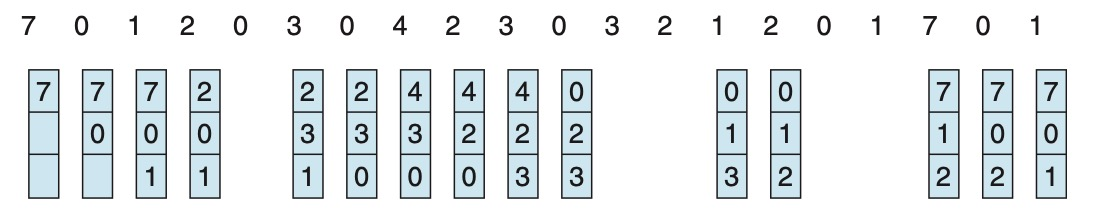
\includegraphics[width=0.5\linewidth]{assets/FIFO-paging-ex.jpg}
    \caption{Example when usign a 3 frame memory}
\end{figure}

\begin{note}
    Non sempre aumentare le dimensioni della memoria porta ad una riduzione del numero di page fault, questo fatto è noto come \textit{Anomalia di Belady}.

    In particolare usando una coda FIFO con string dei riferimenti 1 2 3 4 1 2 5 1 2 3 4 5
    \begin{figure}[H]
        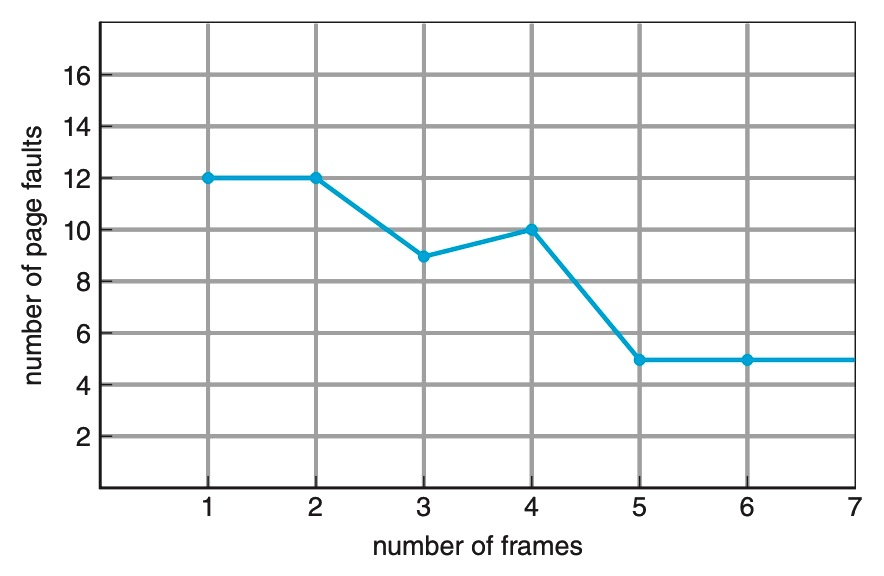
\includegraphics[width=0.4\linewidth]{assets/anomalia-belady.jpeg}
    \end{figure}
\end{note}

\subsubsection{LRU}
L'algoritmo rimpiazza la pagina che non è stata utilizzata per più tempo, provando a prevedere il futuro conoscendo il passato.

Questo algoritmo genera 12 page fault sulla stringa di riferimento.

\spacer
LRU viene considerato un buon algoritmo per questa applicazione, tuttavia risulta esserne difficile l'implementazione. Ci sono diverse soluzioni per l'implementazione, ma tutte richiedono dell'hardware dedicato per renderle praticabili.

\subsubsection{LFU}
Least Frequently Used, si rimpiazza la pagina meno utilizzata.

\subsubsection{MFU}
Most Frequently Used, si basa sull'idea che la pagina utilizzata più di recente non deve essere ricopiata in memoria per essere rimpiazzata.

\subsubsection{Seconda Chance}
L'algoritmo si basa su un algoritmo FIFO, ma viene aggiunto un bit di riferimento ad ogni pagina.

Il bit di riferimento di tutte le pagine viene inizialmente impostato a 0, quando vengono utilizzate viene impostato ad 1.

\spacer
Quando è necessario sostituire una pagina si cerca nella coda FIFO, se si incontra uno 0 quella pagina verrà rimossa. Altrimenti se si incontra un 1 si dà alla pagina una seconda chance, impostando il bit a 0 e spostandosi oltre.

\begin{figure}[H]
    \centering
    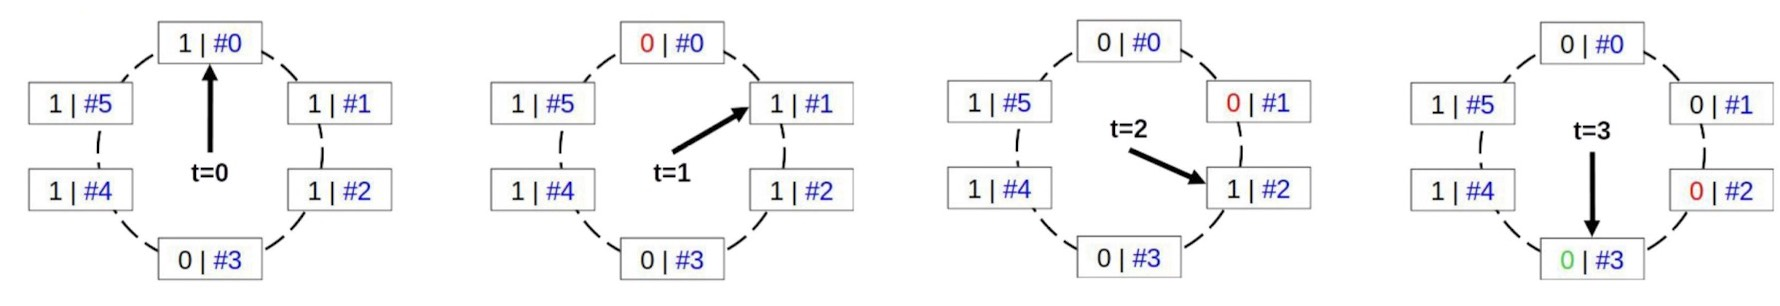
\includegraphics[width=0.9\linewidth]{assets/algoritmo-seconda-chance.jpg}
\end{figure}

L'algoritmo può essere migliorato tenendo conto anche del bit di modifica, si consideri la coppia (bit di riferimento, bit di modifica).

La pagina migliore è quella con valore (0, 0), seguita da (0, 1) che ha il difetto di dover essere salvata sulla memoria secondaria.

\subsubsection{Pool di Frame Liberi}
L'algoritmo richiede che venga sempre mantenuto un certo numero di frame liberi in memoria. Questi vengono utilizzati da buffer, dopo la selezione del frame vittima il nuovo frame viene scritto in uno dei frame liberi e infine il frame vittima viene copiato in memoria secondaria.

\spacer
Un'altra ottimizzazione disponibile è quella di controllare la memoria secondaria e quando esso è inattivo utilizzarlo per copiare dei frame modificati, resettando il loro bit di modifica.

\subsection{Allocazione dei Frame}
Il numero minimo di pagine che viene allocato ad un processo è deciso dall'architettura, mentre il massimo è dettato dalla dimensione della memoria primaria.

\subsubsection*{Allocazione Uniforme}
Semplicemente divide lo spazio della memoria per i programmi in esecuzione, quindi se si hanno 100 frame e 5 processi ognuno otterrà 20 frame.

\subsubsection*{Allocazione Proporzionale}
Uno schema di allocazione proporzionale alla dimensione del processo, un processo con più frame riceverà più risorse.

\subsubsection*{Allocazione con Priorità}
Si impiega uno schema basato sulla priorità, questa stessa priorità viene utilizzata anche per la scelta dei frame da rimuovere, un processo a priorità maggiore rimuoverà frame di processi a priorità inferiore.

\subsubsection*{Allocazione locale e globale}
L'allocazione globale permette ai processi di prendere frame da qualsiasi altro processo in esecuzione, quella locale invece limita le scelte ai frame che appartengono già al processo.

\spacer
Nei sistemi moderni si preferisce l'allocazione globale in quanto spesso garantisce un numero minore di page fault.

\subsection{Mappatura di File}
La mappatura di file in memoria permette l'accesso in modo completamente simile a quanto si fa per qualsiasi altro dato, l'accesso iniziale avviene tramite un page fault grazie al quale viene copiata una pagina di dati alla memoria principale.

\spacer
Questo permette anche di condividere il file tra più programmi in modo semplice dato che si trova in memoria virtuale.

Purtroppo ci sono anche degli svantaggi, legati principalmente a mantenere l'integrità del file anche in presenza di concorrenza.
\spacer
Il file viene aggiornato effettivamente in memoria solo alla chiusura o quando il pager decide di resettare il bit di modifica.

\spacer
Tutti i moderni sistemi operativi supportano la mappatura di file in memoria principale, spesso tramite una chiamata di sistema (\texttt{mmap()}).
Alcuni sistemi utilizzano la mappatura di default, come Solaris, rimuovendo così l'overhead causato dalla system call.

\subsubsection{Mappatura dell'I/O}
È possibile condividere informazioni tra processo e dispositivo I/O grazie alla mappatura in memoria, ad esempio un processo può scrivere su degli indirizzi di memoria, dai quali la scheda video prenderà i dati da mostrare all'utente.

\subsubsection{Copy On Write}
Le pagine di memoria vengono condivise tra due o più processi, quando uno vuole scrivere su una pagina la copia prima in una nuova locazione di memoria e poi la modifica.

\begin{figure}[H]
    \centering
    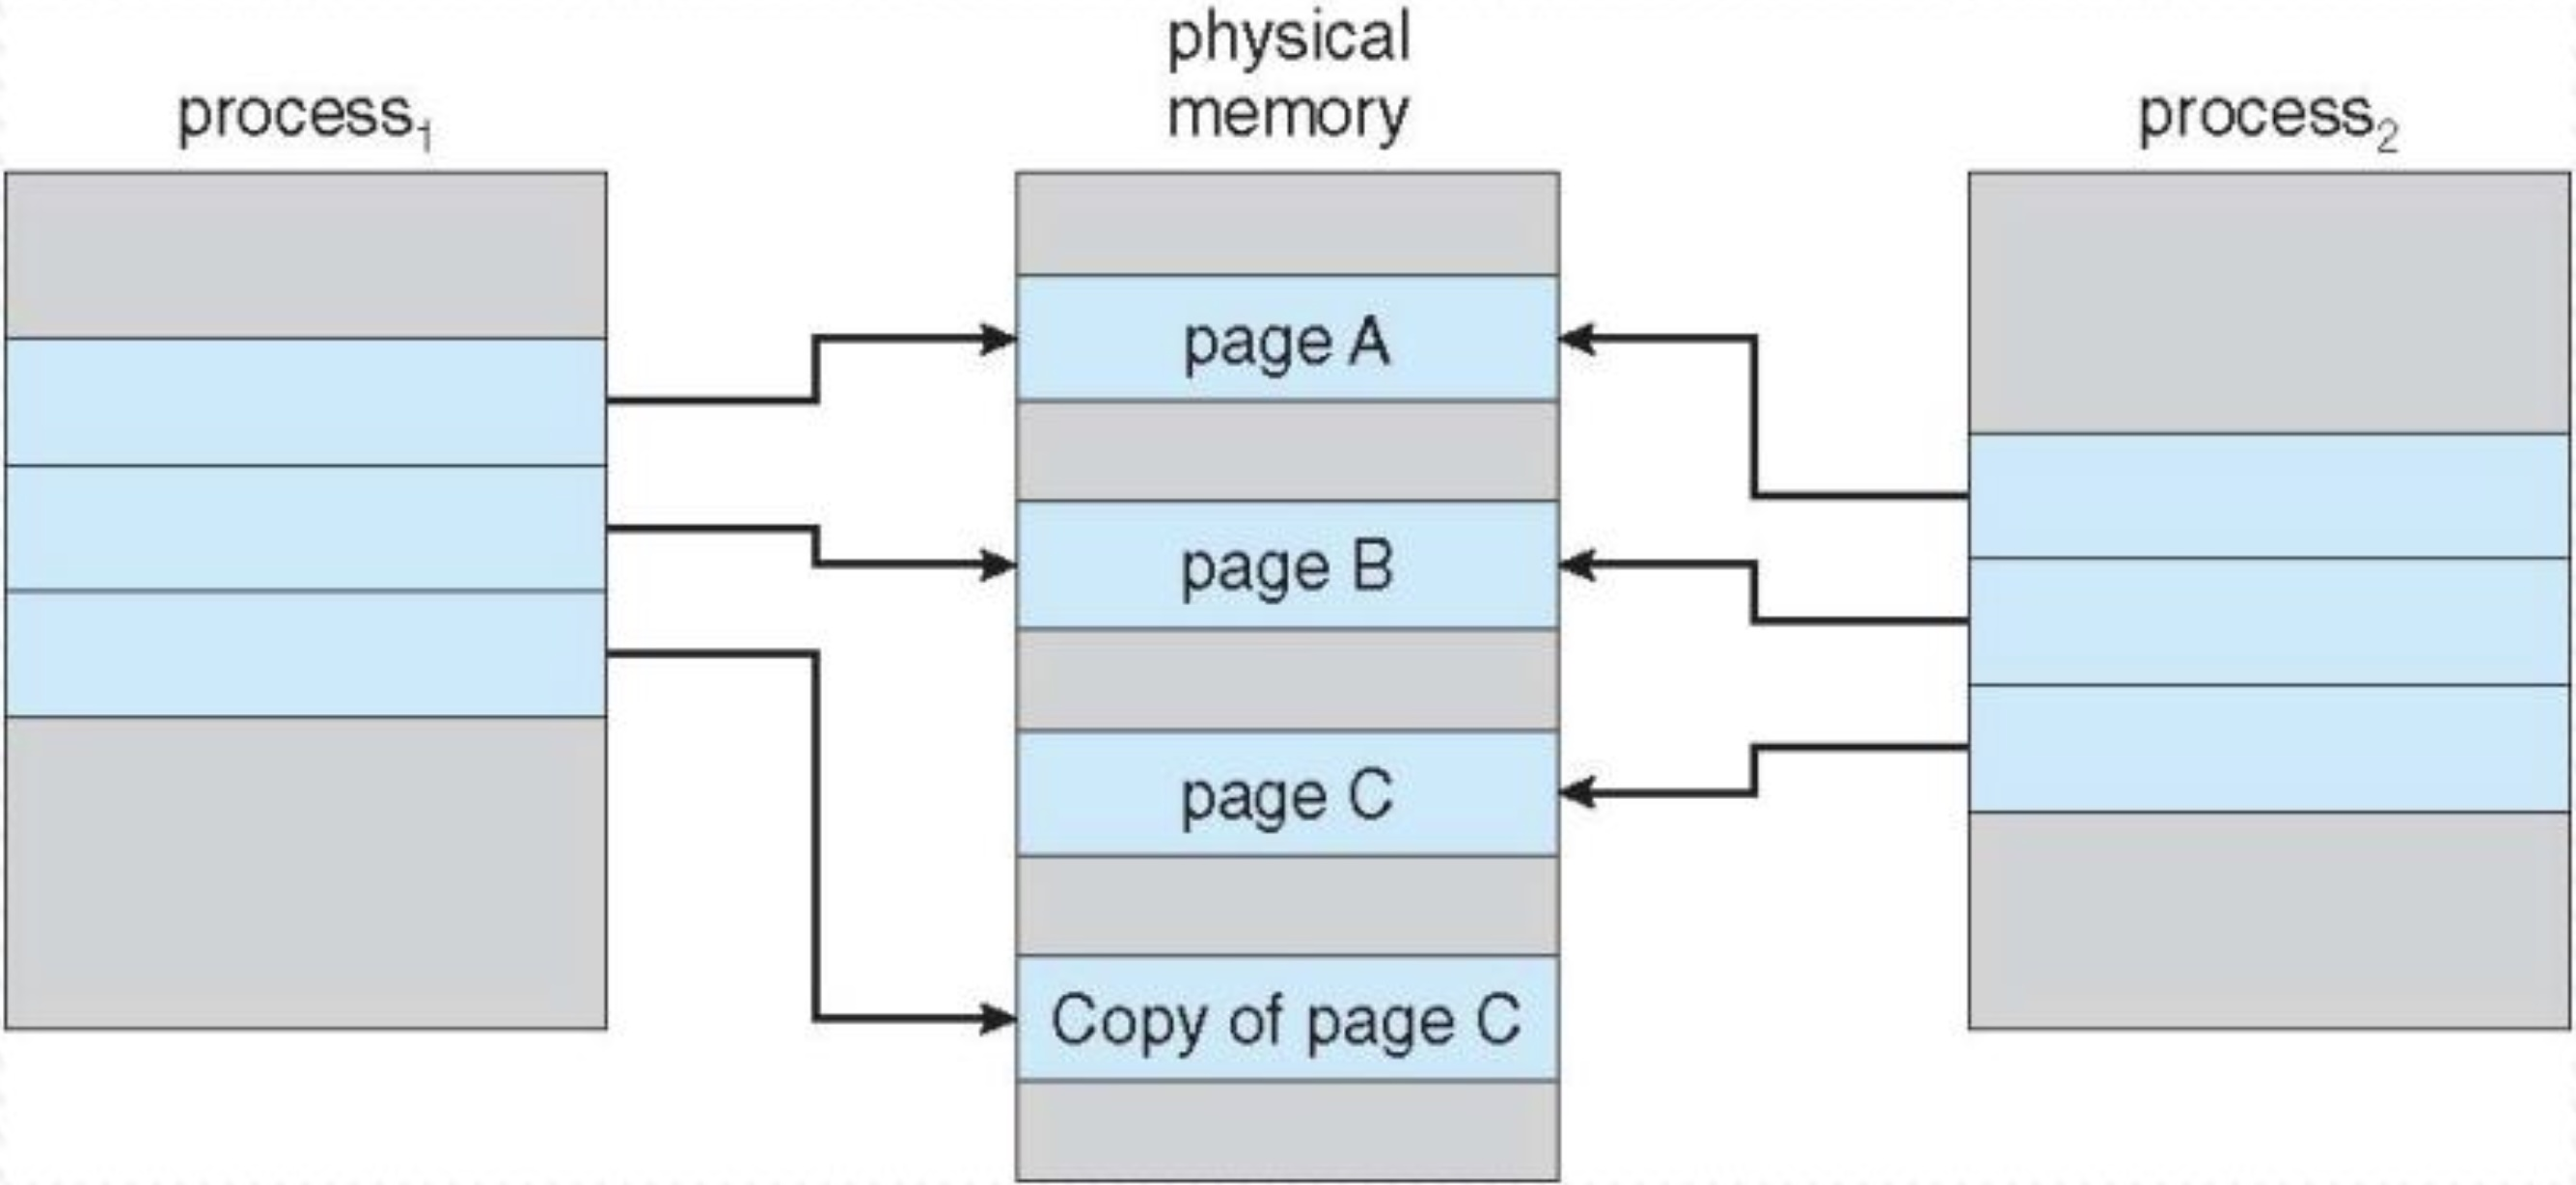
\includegraphics[width=0.5\linewidth]{assets/copy-on-write.jpeg}
\end{figure}

\section{Trashing}
Definiamo trashing la situazione in cui un processo è costantemente occupato a spostare pagine dal disco al posto di utilizzare le risorse del processore.

\spacer
Possiamo dire che c'è un certo numero di processi oltre il quale la multiprogrammazione diventa uno spreco di risorse, in quanto viene perso troppo tempo in page fault.
\begin{figure}[H]
    \centering
    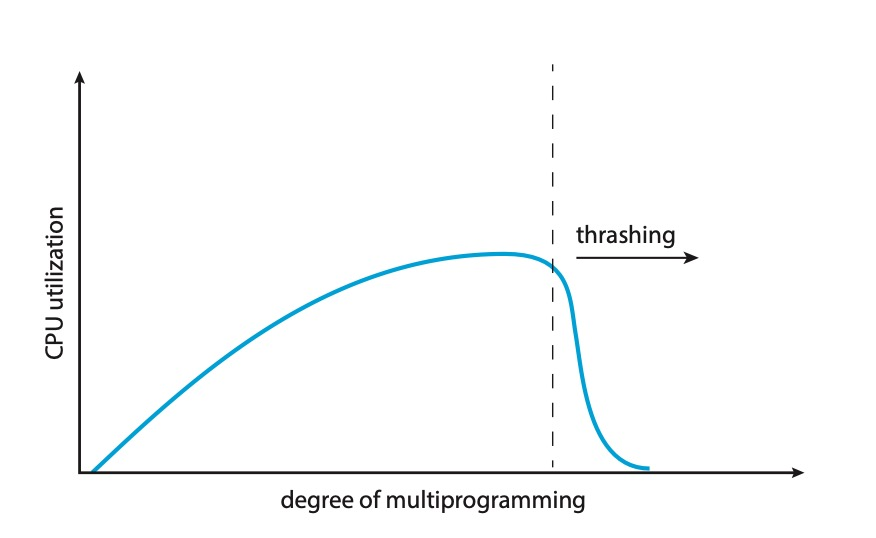
\includegraphics[width=0.4\linewidth]{assets/trashing.jpg}
\end{figure}

Vogliamo quindi trovare il massimo numero di processi che possiamo eseguire in multiprogrammazione senza incorrere nel \textit{trashing}, per decidere questo utilizziamo il modello di località.

Il modello afferma che un processo si sposta da una località ad un'altra durante la sua esecuzione, una località è un insieme di indirizzi che sono spesso utilizzati insieme.

\subsection{Working Set}
Possiamo approssimare la località di un processo guardando ai frame che esso ha utilizzato nelle ultime $\Delta$ chiamate alla memoria, chiamiamo il set dei frame usati dal processo $i$ nel periodo $\Delta$ \textit{Working Set ($WSS_i$)} .

\begin{note}
    $\Delta$ deve essere della giusta dimensione, troppo piccolo e non conterrà tutta la località, troppo grande e conterrà più località
\end{note}

Rappresentiamo il Working set con due numeri: $WS(t, \Delta)$ dove il primo è l'istante che stiamo analizzando, mentre il secondo la dimensione della località.

Otteniamo quindi $D = \sum_i WSS_i$, il numero totale di frame attualmente nella località dei processi in esecuzione, se questo numero supera il numero totale dei frame disponibili nella memoria principale si rischia di incorrere nel \textit{trashing}.

A questo punto è conveniente terminare alcuni processi o sottoporli a swapping.

\spacer
Il working set è un insieme in constante cambiamento, quindi per alleggerirne l'utilizzo è conveniente effettuare il controllo su un determinato periodo e salvare quali frame sono presenti in almeno un working set in un bit di stato (1 se presente, 0 se non presente).

Quando sarà necessario rimuovere un frame si cercherà quello con il maggior numero di 0 nei suoi bit di stato, ovvero quello che non appare nei working set da più tempo.

\subsection{Frequenza di Page Fault}
Un approccio più diretto è quello di stabilire una certa frequenza di page fault "accettabile" e aumentare o diminuire i frame di conseguenza.

\begin{figure}[H]
    \centering
    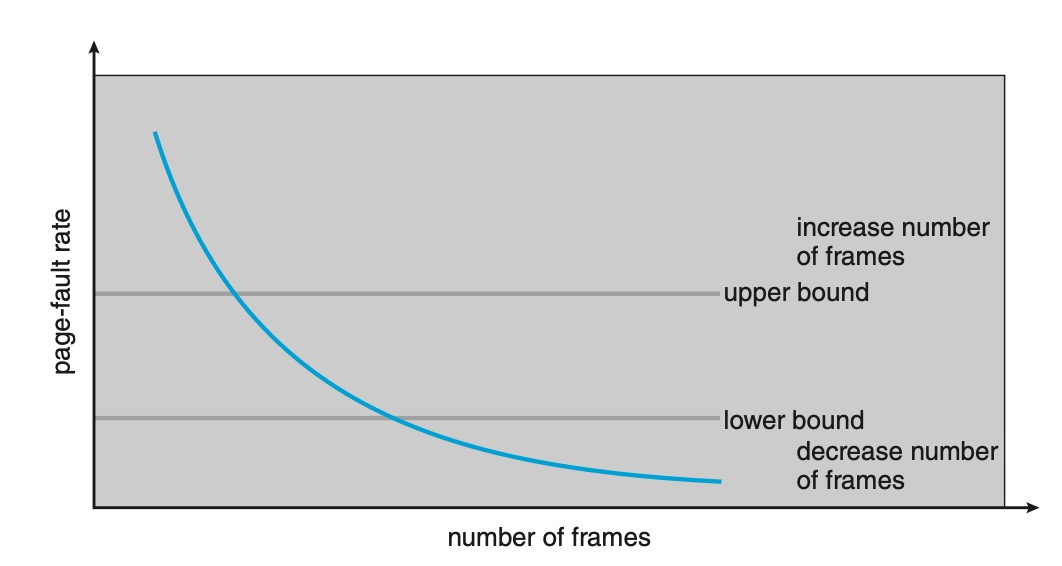
\includegraphics[width=0.5\linewidth]{assets/frequenza-page-fault.jpg}
\end{figure}

\subsection{Relazione tra Working Set e Frequenza di Page Fault}
Il cambiamento di località comporta un picco di page fault

\begin{figure}[H]
    \centering
    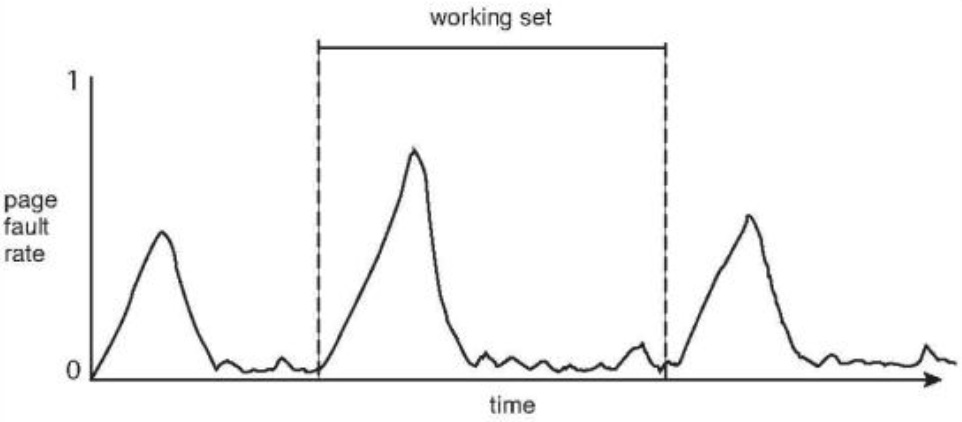
\includegraphics[width=0.5\linewidth]{assets/page-fault-working-set.jpeg}
\end{figure}

\section{Allocazione di Memoria al Kernel}
Il kernel utilizza della memoria separata da quella destinata agli utenti, questa memoria molto spesso non è soggetta a paginazione in quanto esso opera con oggetti di piccole dimensioni che sprecherebbero le pagine.

Inoltre alcune parti della memoria del kernel devono essere contigue per permettere a dispositivi I/O, che non hanno accesso alla memoria fisica, di scriverci.

\spacer
Vedremo ora due tecniche per gestire la memoria che viene riservata al kernel.

\subsection{Allocatore potenza 2}
Utilizza un segmento di memoria a dimensione fissa e fisicamente contigua, che viene allocato in blocchi di dimensione pari a potenze del 2.

\spacer
Quando viene richiesta una quantità di memoria essa viene arrotondata alla più piccola potenza che la contiene, se si richiede una quantità di memoria minore il segmento viene diviso a metà.

\begin{figure}[H]
    \centering
    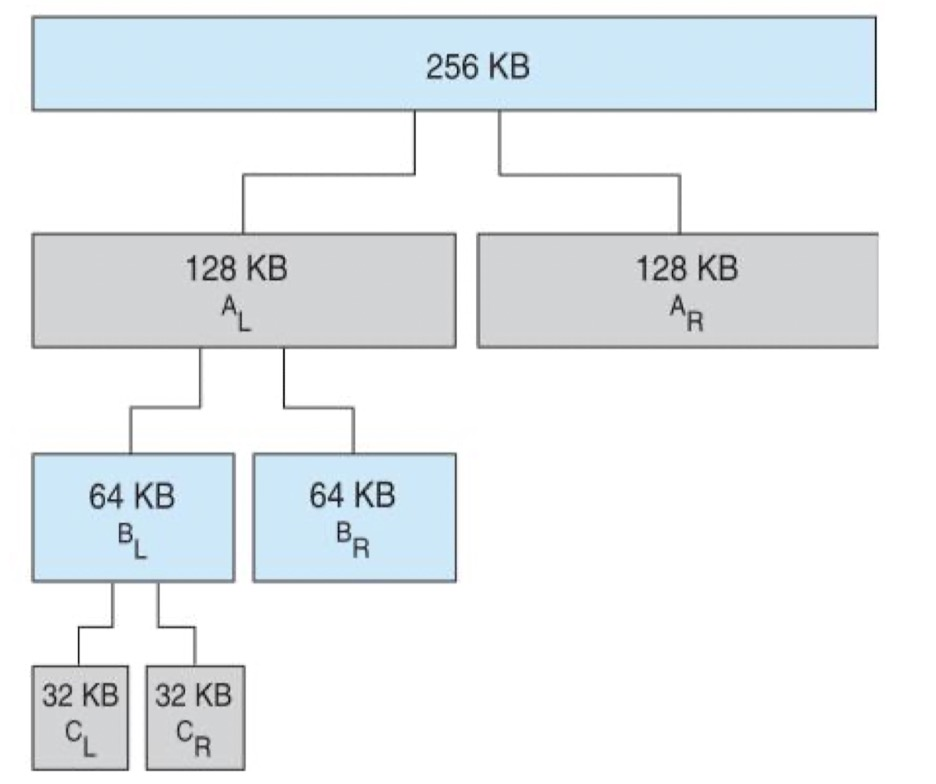
\includegraphics[width=0.4\linewidth]{assets/allocatore-potenza-2.jpg}
\end{figure}

\subsection{Allocazione a Lastra}
Il kernel ha la necessità di allocare e distruggere oggetti frequentemente, per questo motivo è conveniente mantenere una cache per ogni tipo di oggetto così da rimuovere il costo di inizializzazione.

\spacer
Le cache contengono istanze della struttura dati del kernel a cui sono assegnate e vengono inserite in una lastra (\textit{slab}), dei segmenti di memoria fisicamente contigui.

\spacer
Quando il kernel richiede un nuovo oggetto esso viene preso da quelli segnati come liberi.

Se non dovessero essere disponibili oggetti liberi ne vengono allocati altri in una lastra vuota. Nel caso in cui non dovessero esserci lastre libere verrà allocato spazio per far crescere la cache di una lastra.

\begin{figure}[H]
    \centering
    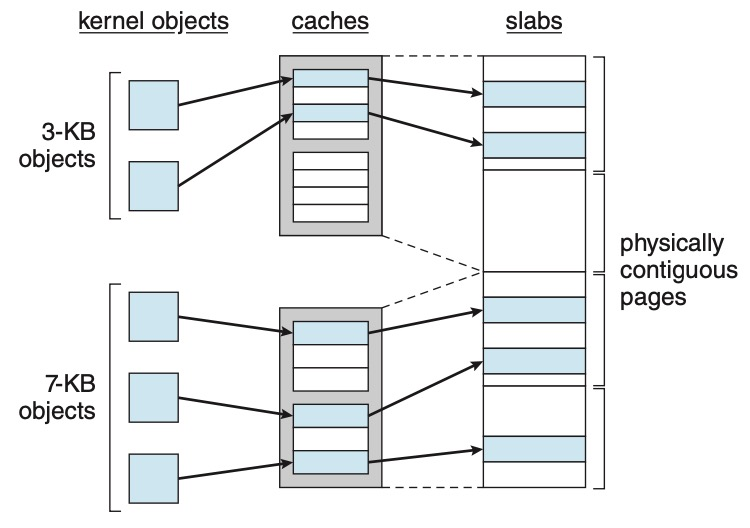
\includegraphics[width=0.5\linewidth]{assets/allocatore-lastra.jpg}
\end{figure}

\section{Implementazioni}
\subsection{Linux}
Per quanto riguarda la \textbf{Memoria del Kernel} linux utilizza il sistema Buddy, un allocatore potenza di 2.
Invece per le strutture dati, a partire dal kernel 2.4, viene utilizzato l'allocatore SLOB o SLUB.
\begin{sitemize}
    \item \textbf{SLOB:} Utilizzato per sistemi con poca memoria, mantiene 3 liste, per oggetti grandi, medi e piccoli.
    \item \textbf{SLUB:} Allocatore a lastre ottimizzata per sistemi multicore.
\end{sitemize}

\spacer
Invece la \textbf{Memoria Utente} viene gestita tramite paginazione su richiesta.
La politica di sostituzione è detta Clock: vengono mantenute due liste, \texttt{active\_list} e \texttt{inactive\_list}, la prima che contiene le pagine in uso e la seconda contiene pagine non utilizzate di frequente che possono essere rimosse.

\spacer
Ogni pagina ha un bit di accesso.
\begin{sitemize}
    \item Quando una pagina viene \textbf{allocata} o \textbf{riferita} il bit viene impostato su 1 e viene inserita in coda a \texttt{active\_list}.
    \item La pagina utilizzata meno di recente si sposta in testa alla lista \texttt{active\_list}, dalla quale viene \textbf{spostata} verso la lista \texttt{inactive\_list} per mantenere le due liste bilanciate.
    \item Inoltre i bit di accesso vengono resettati periodicamente, riportando il sistema ad uno stato iniziale con tutti i processi in \texttt{inactive\_list}.
    \item Il deamon \texttt{kswapd} si risveglia periodicamente e se la memoria non è sufficiente \textbf{termina} dei programmi dalla \texttt{inactive\_list}.
\end{sitemize}

\subsection{Windows}
Per quanto riguarda la \textbf{Memoria del Kernel} Windows scrive i dati su un page file, ma quando questo non è possibile i dati vengono scritti su una pool di memoria non paginata. (ad es. quando Windows non può fare page fault perché sta gestendo un page fault.)

\spacer
Invece la \textbf{Memoria Utente} viene gestita tramite paginazione con clustering, quindi quando avviene un page fault viene caricato non solo la pagina richiesta, ma anche le pagine adiacenti.

Ad un processo viene assegnato una dimensione minima e massima del working set, il minimo è il numero di pagine garantite dal sistema operativo, il numero massimo è il limite oltre il quale il processo non può allocare.

Quando l'occupazione della memoria scende si effettua una riassegnazione dei working set aumentando i tetti massimi per processo.

\spacer
Windows fa inoltre uso di compressione delle pagine più vecchie, prima di ricorrere alla memoria virtuale. Quando poi i dati tornano ad essere utilizzati devono prima essere decompressi.

